\documentclass[a4paper,landscape]{article}

\usepackage[landscape,top=0cm,left=0cm,bottom=0cm,right=0cm]{geometry}
\usepackage{tikz}
\usepackage{background}
\usepackage{blindtext}
\usetikzlibrary{matrix, shapes.misc, calc}

\pagestyle{empty}
\setlength{\parindent}{0cm}

\begin{document}

@foreach($children as $chunk)
    \backgroundsetup{scale = 1, angle = 0, opacity = 1, color=black, contents = {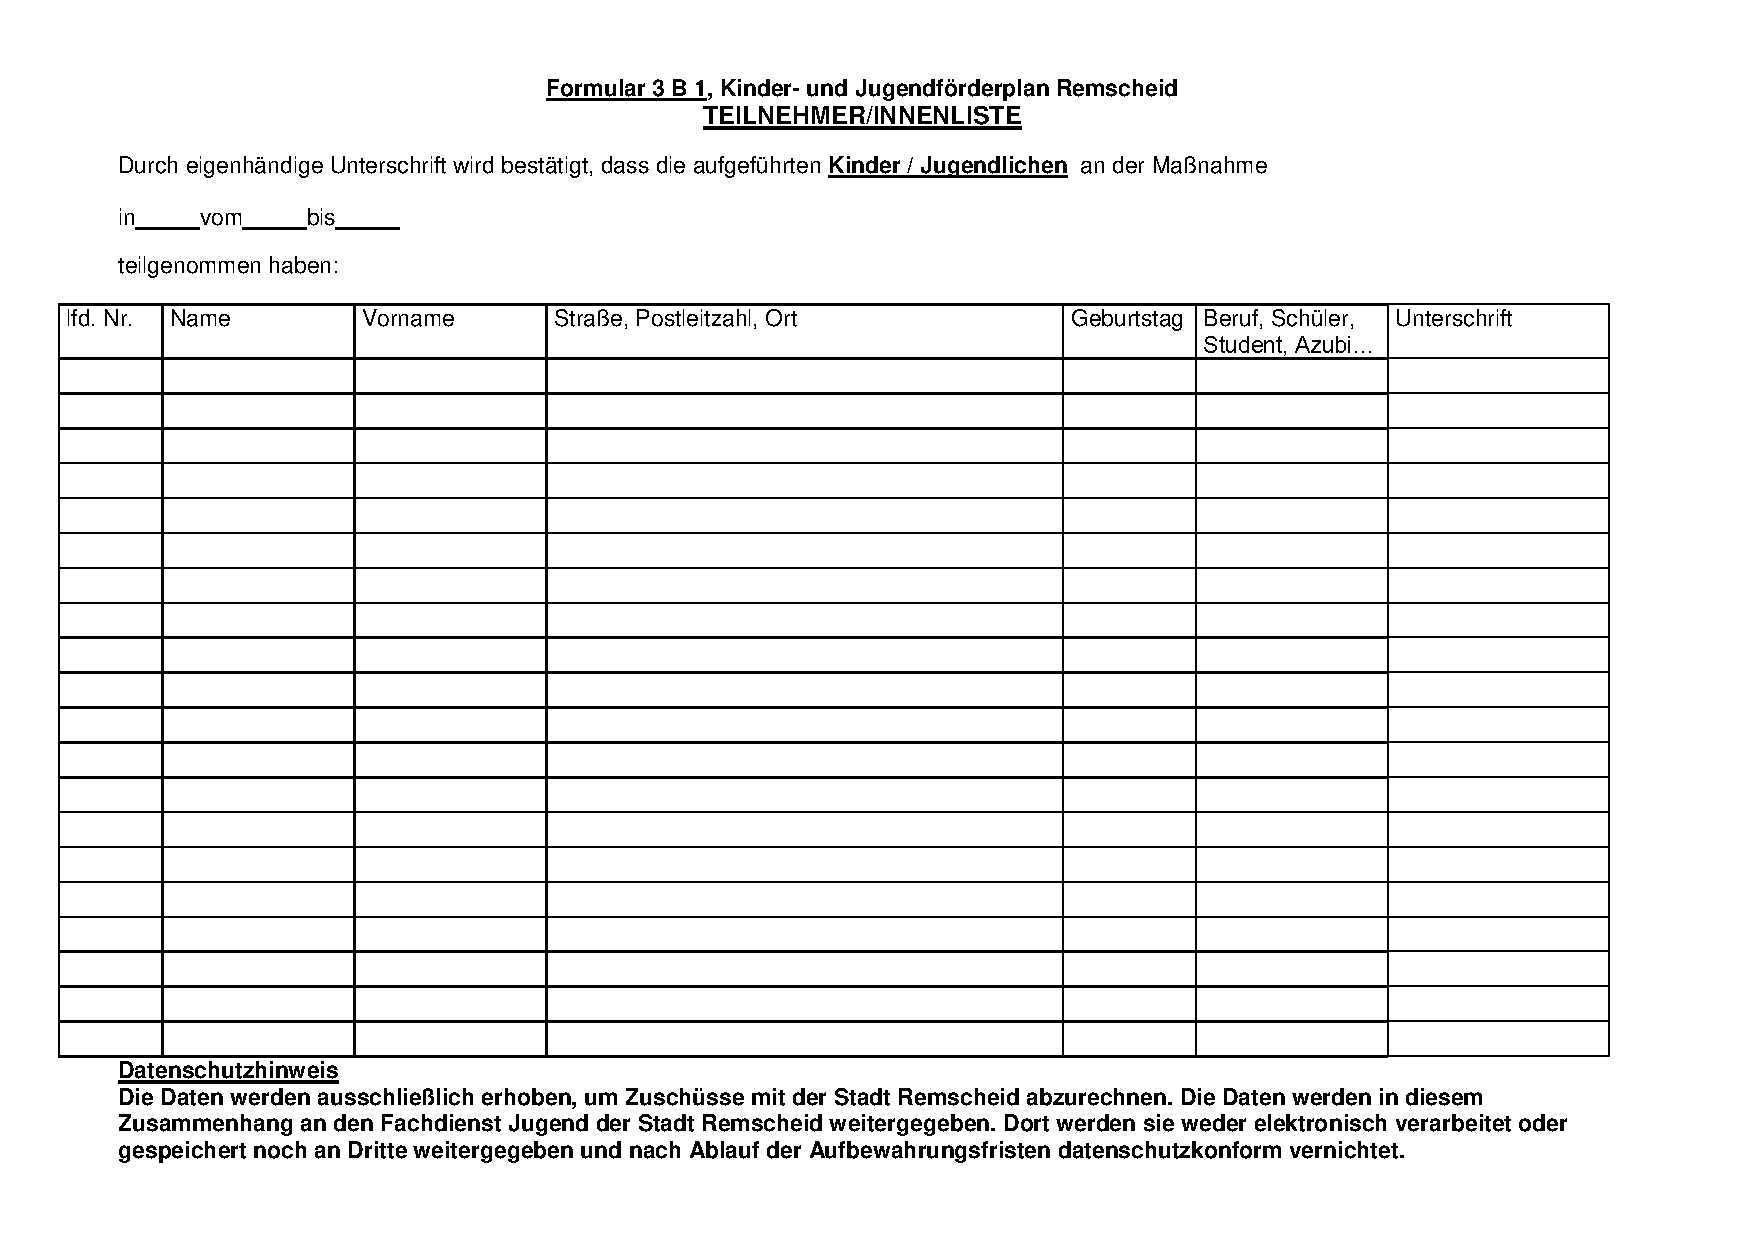
\includegraphics[width = \paperwidth, height = \paperheight] {tn.pdf}}}
    \noindent \sffamily
    \begin{tikzpicture}[remember picture,overlay,yscale=-1]
        \fill[white] (19mm,30mm) rectangle (80mm,36mm);
        \node[anchor=base west,fill=white] at (18.8mm,34mm) {\large{In \textbf{<<<$zipLocation>>>} vom \textbf{<<<$niceDateFrom>>>} bis \textbf{<<<$niceDateUntil>>>}}};

        @foreach($chunk as $i => $member)
            \node[anchor=base, text width=7.75mm, align=center] at ($(18.35mm, 61.3mm + 5.91mm * <<<$i % 20>>>)$) {<<<$i+1>>>};
            \node[anchor=base, text width=29mm, align=center] at ($(43.7mm, 61.3mm + 5.91mm * <<<$i % 20>>>)$) {<<<$member->lastname>>>};
            \node[anchor=base, text width=29mm, align=center] at ($(76.2mm, 61.3mm + 5.91mm * <<<$i % 20>>>)$) {<<<$member->firstname>>>};
            \node[anchor=base, text width=84mm, align=center] at ($(136.2mm, 61.3mm + 5.91mm * <<<$i % 20>>>)$) {<<<$member->fullAddress>>>};
            \node[anchor=base, text width=19mm, align=center] at ($(191.2mm, 61.3mm + 5.91mm * <<<$i % 20>>>)$) {<<<$member->birthday->format('d.m.Y')>>>};
        @endforeach
    \end{tikzpicture}

    \pagebreak
@endforeach

@foreach($leaders as $chunk)
    \backgroundsetup{scale = 1, angle = 0, opacity = 1, color=black, contents = {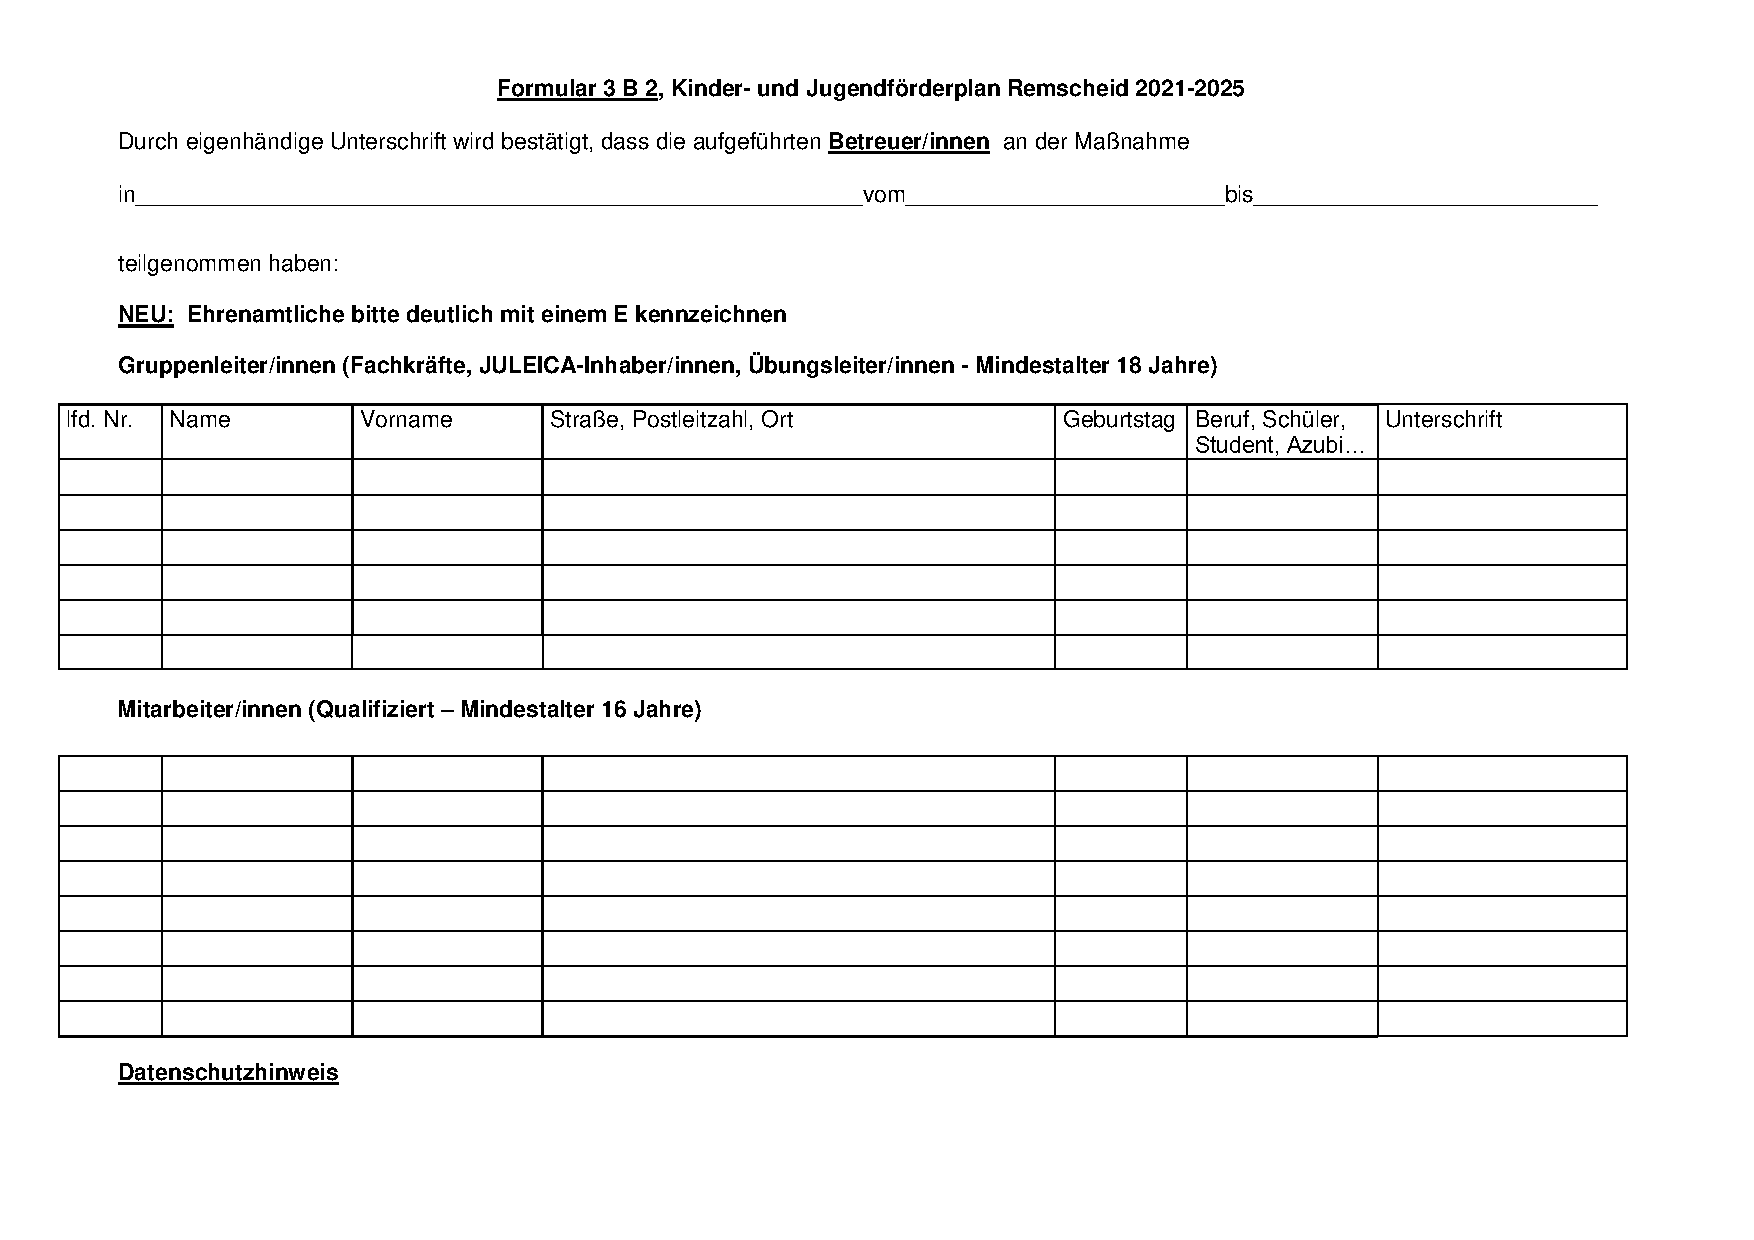
\includegraphics[width = \paperwidth, height = \paperheight] {leader.pdf}}}
    \noindent \sffamily
    \begin{tikzpicture}[remember picture,overlay,yscale=-1]
        \fill[white] (17mm,27mm) rectangle (284mm,34mm);
        \node[anchor=base west,fill=white] at (18.8mm,32mm) {\large{In \textbf{<<<$zipLocation>>>} vom \textbf{<<<$niceDateFrom>>>} bis \textbf{<<<$niceDateUntil>>>}}};

        @foreach($chunk as $i => $member)
            \node[anchor=base, text width=7.75mm, align=center] at ($(18.35mm, 78.3mm + 5.91mm * <<<$i % 6>>>)$) {<<<$i+1>>>};
            \node[anchor=base, text width=29mm, align=center] at ($(43.7mm, 78.3mm + 5.91mm * <<<$i % 6>>>)$) {<<<$member->lastname>>>};
            \node[anchor=base, text width=29mm, align=center] at ($(76.2mm, 78.3mm + 5.91mm * <<<$i % 6>>>)$) {<<<$member->firstname>>>};
            \node[anchor=base, text width=84mm, align=center] at ($(136.2mm, 78.3mm + 5.91mm * <<<$i % 6>>>)$) {<<<$member->fullAddress>>>};
            \node[anchor=base, text width=19mm, align=center] at ($(190.2mm, 78.3mm + 5.91mm * <<<$i % 6>>>)$) {<<<$member->birthday->format('d.m.Y')>>>};
        @endforeach
    \end{tikzpicture}

    \pagebreak
@endforeach

\end{document}



